\begin{figure}[h!]
	\centering
	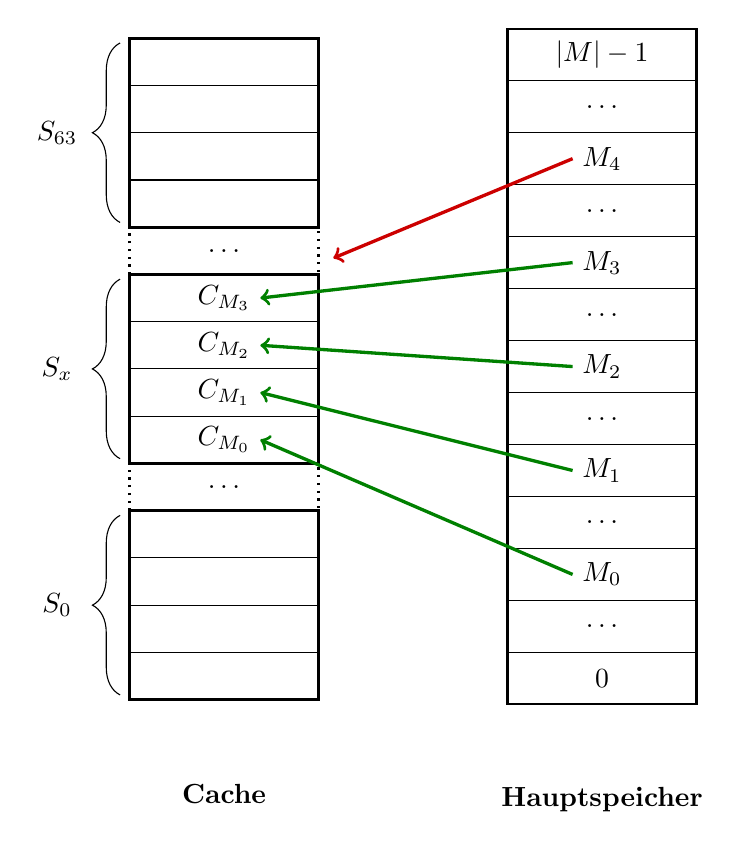
\begin{tikzpicture}[scale=0.6]
% === Cache ===
%Set 0
\draw[] (0,0) rectangle (4,1);
\draw[] (0,1) rectangle (4,2);
\draw[] (0,2) rectangle (4,3);
\draw[] (0,3) rectangle (4,4);
%Label
\draw[very thick] (0,0) rectangle node[yshift=-2.4cm] () {\textbf{Cache}}(4,4);
%Klammer
\draw [decorate,decoration={brace,amplitude=10pt}]
(-0.2,0.1) -- (-0.2,3.9) node [black,midway,xshift=-0.8cm] {$S_0$};




%Lücke
\draw[dotted, thick] (0,4) rectangle node[] {\textbf{$\dots$}} (4,5);

%Set X
\draw[] (0,5) rectangle node[] (c1) {\textbf{$C_{M_0}$}} (4,6);
\draw[] (0,6) rectangle node[] (c2) {\textbf{$C_{M_1}$}} (4,7);
\draw[] (0,7) rectangle node[] (c3) {\textbf{$C_{M_2}$}} (4,8);
\draw[] (0,8) rectangle node[] (c4) {\textbf{$C_{M_3}$}} (4,9);
\draw[very thick] (0,5) rectangle node[yshift=1.35cm, xshift=1.25cm] (set) {} (4,9);
%Klammer
\draw [decorate,decoration={brace,amplitude=10pt}]
(-0.2,5.1) -- (-0.2,8.9) node [black,midway,xshift=-0.8cm] {$S_x$};

%Lücke
\draw[dotted, thick] (0,9) rectangle node[] {\textbf{$\dots$}} (4,10);

%Set 63
\draw[] (0,10) rectangle (4,11);
\draw[] (0,11) rectangle (4,12);
\draw[] (0,12) rectangle (4,13);
\draw[] (0,13) rectangle (4,14);
\draw[very thick] (0,10) rectangle (4,14);
%Klammer
\draw [decorate,decoration={brace,amplitude=10pt}]
(-0.2,10.1) -- (-0.2,13.9) node [black,midway,xshift=-0.8cm] {$S_{63}$};

% === Hauptspeicher ===
\draw[] (8,-0.1) rectangle node[]      {\textbf{$0$}}     (12, 1.0);
\draw[] (8, 1.0) rectangle node[]      {\textbf{$\dots$}} (12, 2.1);
\draw[] (8, 2.1) rectangle node[] (m1) {\textbf{$M_0$}}     (12, 3.2);
\draw[] (8, 3.2) rectangle node[]      {\textbf{$\dots$}} (12, 4.3);
\draw[] (8, 4.3) rectangle node[] (m2) {\textbf{$M_1$}}     (12, 5.4);
\draw[] (8, 5.4) rectangle node[]      {\textbf{$\dots$}} (12, 6.5);
\draw[] (8, 6.5) rectangle node[] (m3) {\textbf{$M_2$}}     (12, 7.6);
\draw[] (8, 7.6) rectangle node[]      {\textbf{$\dots$}} (12, 8.7);
\draw[] (8, 8.7) rectangle node[] (m4) {\textbf{$M_3$}}     (12, 9.8);
\draw[] (8, 9.8) rectangle node[]      {\textbf{$\dots$}} (12,10.9);
\draw[] (8,10.9) rectangle node[] (m5) {\textbf{$M_4$}}     (12,12.0);
\draw[] (8,12.0) rectangle node[]      {\textbf{$\dots$}} (12,13.1);
\draw[] (8,13.1) rectangle node[]      {\textbf{$|\mathbb{M}|-1$}} (12,14.2);
\draw[thick] (8,-0.1) rectangle node [yshift=-5.5cm] () {\textbf{Hauptspeicher}} (12,14.2);

%Pfeile	
\draw[black!50!green, ->, very thick] (m1.west) -- (c1.east);
\draw[black!50!green, ->, very thick] (m2.west) -- (c2.east);
\draw[black!50!green, ->, very thick] (m3.west) -- (c3.east);
\draw[black!50!green, ->, very thick] (m4.west) -- (c4.east);
\draw[black!20!red, ->, very thick] (m5.west) -- (set);
	\end{tikzpicture}
	\caption{Belegung eines Cache-Sets durch \texttt{crpi}}
	\label{cacheLayout}
\end{figure}
